% Part: sets-functions-relations
% Chapter: relations
% Section: graphs

\documentclass[../../../include/open-logic-section]{subfiles}

\begin{document}

\olfileid{sfr}{rel}{grp}
\olsection{Graphs}

Un \emph{grafo} es un diagrama en el que los puntos—llamados ``nodos'' o ``vértices'' (plural de ``vértice'')—están conectados por aristas. Los grafos son una herramienta ubicua en matemáticas discretas y en ciencias de la computación. Son increíblemente útiles para representar y visualizar relaciones y estructuras, desde cosas concretas como redes de diversos tipos hasta estructuras abstractas como los posibles resultados de decisiones. Existen muchos tipos diferentes de grafos en la literatura que difieren, por ejemplo, según si las aristas están dirigidas o no, tienen etiquetas o no, si puede haber aristas desde un nodo al mismo nodo, múltiples aristas entre los mismos nodos, etc. Los \emph{grafos dirigidos} tienen una conexión especial con las relaciones.

\begin{defn}[Grafo dirigido]
Un \emph{grafo dirigido} $G = \tuple{V, E}$ es un conjunto de \emph{vértices}~$V$ y un conjunto de \emph{aristas}~$E \subseteq V^2$.
\end{defn}

\begin{explain}
Según nuestra definición, un grafo es simplemente un conjunto junto con una relación en ese conjunto. Por supuesto, al hablar de grafos, es natural esperar que estén representados gráficamente: podemos dibujar un grafo conectando dos vértices~$v_1$ y $v_2$ mediante una flecha si y solo si $\tuple{v_1, v_2} \in E$. La única diferencia entre una relación por sí misma y un grafo es que un grafo especifica el conjunto de vértices, es decir, un grafo puede tener vértices aislados. El punto importante, sin embargo, es que cada relación~$R$ en un conjunto~$X$ puede verse como un grafo dirigido $\tuple{X, R}$, y, a la inversa, un grafo dirigido~$\tuple{V, E}$ puede verse como una relación $E \subseteq V^2$ con el conjunto $V$ especificado explícitamente.
\end{explain}

\begin{ex}
El grafo $\tuple{V, E}$ with $V = \{1, 2, 3, 4\}$ y $E =
\{\tuple{1,1}, \allowbreak \tuple{1, 2}, \allowbreak \tuple{1, 3},
\allowbreak \tuple{2, 3}\}$ se ve así:
\begin{align*}
& 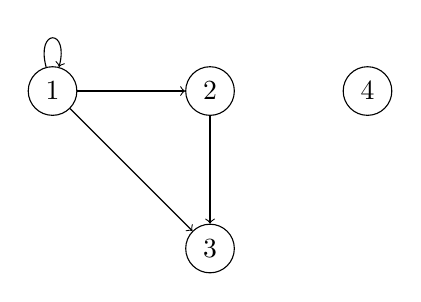
\begin{tikzpicture}[->,node distance=2cm]
  \node[draw,circle] (A) {$1$};
  \node[draw,circle] (B) [right of=A] {$2$};
  \node[draw,circle] (C) [below of=B] {$3$};
  \node[draw,circle] (D) [right of=B] {$4$};
  \draw (A) to [loop above]  (A);
  \draw (A) to  (B);
  \draw (A) to  (C);
  \draw (B) to  (C);
  \end{tikzpicture}
\intertext{Este es un grafo diferente a $\tuple{V', E}$ con $V' =
  \{1, 2, 3\}$, el cual luce así:}
& 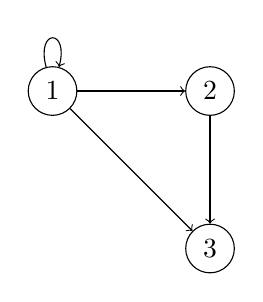
\begin{tikzpicture}[->,node distance=2cm]
  \node[draw,circle] (A) {$1$};
  \node[draw,circle] (B) [right of=A] {$2$};
  \node[draw,circle] (C) [below of=B] {$3$};
  \draw (A) to [loop above]  (A);
  \draw (A) to  (B);
  \draw (A) to  (C);
  \draw (B) to  (C);
  \end{tikzpicture}
\end{align*}
\end{ex}

\begin{prob}
  Consideremos la relación menor-o-igual que ~$\le$ en el conjunto $\{1,
  2, 3, 4\}$ en forma de gráfico y dibuja el diagrama correspondiente.
\end{prob}

\end{document}
